%----------------------------------------------------------------------
%                        PROJECT DEFINITION
%----------------------------------------------------------------------
\renewcommand{\projnr}{D1}
\renewcommand{\projtitleshort}{Radioisotope chronometry}
\renewcommand{\projauth}{Trieloff, Altherr}
%
\setcounter{section}{0}
\noindent{\normalfont\sffamily\Large\bfseries Project \projnr: \projtitleshort}
%
\section{Full title:}
\hspace{1\baselineskip}\\
\centerline{\large ``Radioisotope chronometry and formation of small bodies }
\centerline{in the early solar system''}
%
\section{General information}\mbox{}
\subsection{Principle investigators:}
\hspace{-\baselineskip}\\\noindent
%
{\bfseries\itshape Trieloff}, Mario, Priv. Doz. Dr. \\
non-tenure\\
Date-of-birth: 26.2.63, Nationality: German\\
DFG Code number of latest application: TR333/8-2\\
Mineralogisches Institut der Universit\"at Heidelberg\\
Im Neuenheimer Feld 236\\
69120 Heidelberg\\
Tel: 06221-546022\\
Fax: 06221-544805\\
Email: trieloff@min.uni-heidelberg.de\\
Private address:
Zaystr. 48, 76437 Rastatt
Tel: 07222/151875
%
\vspace{1em}\\\noindent
{\bfseries\itshape Altherr}, Rainer, Prof.~Dr.\\
C4, tenure\\
Date-of-birth: 6.8.47, Nationality: German\\
DFG Code number of latest application: TR333/8-2\\
Mineralogisches Institut der Universit\"at Heidelberg\\
Im Neuenheimer Feld 236\\
69120 Heidelberg\\
Tel: 06221-548206/8207\\
Fax: 06221-544805\\
Email: raltherr@min.uni-heidelberg.de\\
Private address:
Konrad-Adenauer-Str. 2, 69221 Dossenheim
Tel: 06221-866017
%
\vspace{1em}\\\noindent
{\bfseries\itshape Stephan}, Thomas, HDoz. Dr.\\
non-tenure\\
Date-of-birth: 27.2.63, Nationality: German\\
DFG Code number of latest application: Ste 576/17-1\\
Institut f\"ur Planetologie\\
Westf\"alische Wilhelms-Universit\"at M\"unster\\
Wilhelm-Klemm-Stra�e 10\\
48149 M\"unster\\
Tel: 0251-83-39050\\
Fax: 0251-83-36301\\
Email: stephan@uni-muenster.de\\
Private address: Mergelberg 218, 48161 M\"unster
Tel: 0251- 8712880




\subsection{Co-investigators within this Forschergruppe:}
%\begin{coilist}
%\item J.~Blum (IGEP, TU Braunschweig)
%\item G.~Wurm (M\"unster)
%\item S.~Wolf (MPIA Heidelberg)
%\item C.P.~Dullemond (MPIA Heidelberg)



\section{Summary (Zusammenfassung)}
\subsubsection{Summary:} 
Recent chronological studies of meteorite parent body formation in the early
solar system indicate that differentiated planetesimals formed earlier than
chondritic undifferentiated meteorite parent bodies, most probably because
short-lived nuclide heating (mainly $^{26}$Al) triggered planetesimal heating,
leading to differentiation of the planetesimals that formed very early when
$^{26}$Al was more abundant. Formation of chondritic parent bodies 1-4 Ma
after calcium,aluminum-rich inclusions (CAIs) coincides with chondrule
formation ages of 2-3 Ma after CAIs. This observation and chemical
complementarity between chondrules and matrix indicate rapid chondrule
formation just before accretion to chondritic parent bodies, and should
result in strongly peaked age distributions of chondrules of
individual chondrite classes. However, there are other observations that
indicate a larger spread of chondrule ages in the CV chondrite Allende (up
to a few Ma). The age distribution of chondrules of specific chondrite
classes is important for radial mixing time scales of chondrule material in
the solar nebula, and hence for disk models. In this project we shall
investigate chondrule age distributions for selected ordinary and
carbonaceous chondrites. We will check if such age distributions may have
been falsified by secondary isotope reset during later disturbances or
incomplete reset during formation, by applying two chronometers with
different closure temperature, $^{129}$I-$^{129}$Xe and $^{26}$Al-$^{26}$Mg. In an
independent complementary study, radial mixing processes into comet forming
regions are constrained by an ongoing initiative of STARDUST cometary sample
return analysis. The aim is to quantify the fraction of annealed crystalline
or refractory (CAI-like) material with solar-like isotopic composition.

\subsubsection{Zusammenfassung:} 
Neuere chronologische Studien zur Bildung von Meteoriten-Mutterk\"orpern im
fr\"uhen Sonnensystem zeigen, dass sich differenzierte Planetesimale vor
undifferenzierten chondritischen Mutterk\"orpern bildeten. Dies ist
h\"ochstwahrscheinlich auf den Umstand zur\"uckzuf\"uhren, dass die
Aufheizung auf Zerfallsenergie von $^{26}$Al zur\"uckzuf\"uhren ist.
Dadurch konnten sich fr\"uh gebildete Planetesimale mit hohen
26Al-Konzentrationen wesentlich st\"arker aufheizen und differenzieren.  Die
Bildung chondritischer K\"orper 1-4 Ma nach Ca,Al reichen Einschl\"ussen
(CAIs) stimmt mit den Altern einzelner Chondren (2-3 Ma nach CAIs)
\"uberein.  Diese Beobachtung und die sog.\ "chemische Komplementarit\"at"
zwischen Chondren und Matrix weist darauf hin, dass Chondren unmittelbar
nach ihrer Entstehung in die jeweiligen Mutterk\"orper eingebaut wurden
(ohne durch radiale Mischprozesse im solaren Nebel verteilt worden zu
sein). Aufgrund dieses Szenarios erwartet man nur sehr geringe
Altersunterschiede (etwa $<$1 Ma) f\"ur Chondren eines bestimmten
Mutterk\"orpers.  Andere Studien von Chondrenaltern von CV Chondriten zeigen
dagegen Altersunterschiede bis zu einigen Ma. Die Altersverteilung von
Chondren ist daher wichtig f\"ur Zeitskalen f\"ur radiale Mischprozesse im
solaren Nebel und Scheibenmodelle. Innerhalb dieses Projektes sollen
Chondren-Altersverteilungen von gew\"ohnlichen und kohligen Chondriten
untersucht werden. Eine m\"ogliche Verf\"alschung der Bildungsalter durch
unvollst\"andige Zur\"ucksetzung des Isotopensystems oder teilweise
Zur\"ucksetzung durch sp\"atere sekund\"are Ereignisse sollen durch die
Anwendung zweier Chronometer mit unterschiedlichen Schlie{\ss}temperaturen
gepr\"uft werden ($^{129}$I-$^{129}$Xe und $^{26}$Al-$^{26}$Mg).  Ein
unabh\"angiger Teil dieser Studie betrachtet radiale Mischprozesse in die
Regionen, wo sich Kometen gebildet haben. Dazu werden durch ein laufendes
Projekt STARDUST Proben untersucht mit dem Ziel, den Anteil thermisch
ausgeheilter kristalliner oder refrakt\"arer (CAI-\"ahnliche) Materialien
mit solarer Isotopensignatur zu quantifizieren.

\section{State of the art (Stand der Forschung)}
\subsection{Early solar system processes inferred from laboratory analyses of extraterrestrial matter from small solar system bodies}

Two basic processes determine the distribution of condensable matter in
young protoplanetary discs (and, hence, later on the chemistry and structure
of planetary systems and chemical composition of planets): I) chemical
differentiation of the dust component and II) coagulation and eventual
growth to planetesimals and planets. Radial mixing processes (Wooden et
al.\ 2000; Gail et al.\ 2003, 2004; Bockel\'ee-Morvan et al.\ 2002) of matter are
thought to play an important role for disc evolution, particular for
chemical differentiation. While radial transport of planetary matter is also
possible during the late stages of gravitational scattering of planetesimals
and protoplanets (Wetherill \& Steward, 1993; Kokubo \& Ida, 2000), the
diversity of the bulk chemical composition of small chondritic parent bodies
indicates that important chemical differentiation processes (fractionation
of refractory and volatile elements, of Mg-silicates pyroxene/olivine, of
metal and silicate) occurred during the preplanetary phase (e.g.\ Palme
2001). Radial mixing processes can be constrained by demonstrating the mere
occurrence of high temperature products (thermally annealed crystalline
material, high temperature condensates or evaporation residues) that must
have originated from the inner disk and were transported into the outer disc
regions, e.g.\ where comets formed. Time scales of these mixing processes are
difficult to constrain, as the formation time of cometary parent bodies is
not exactly known, and also not the time of annealing of amorphous dust. A
different approach to constrain time scales of radial mixing is to study
solid objects that can be dated by radio-chronometry, and to determine their
lifetimes and radial mixing pathway before they became incorporated into
parent bodies. One example are CAIs: these are the oldest objects in the
solar system, they probably originated close to the sun, and became
incorporated 2-3 Ma later into chondritic parent bodies (Amelin et
al.\ 2002). Another example are chondrules: Some models (Klerner and Palme,
2000) argue that their chemical relationship to matrix components
(``complementarity'') requires that chondrules and matrix formed from the
same precursor material and was rapidly consumed in fast accreting
planetesimals, thereby preventing radial redistribution of chondrules,
independent of their formation process (Scott et al.\ 1996, Desch and
Connolly 2001). If radial mixing processes were active, this would require a
narrow age distribution of chondrules for individual meteorite classes (as
just older chondrules would be removed from the chondrite forming
region). On the other hand, if radial mixing processes were slow, then the
age distribution could comprise older chondrules.  Whatever model applies,
it is clear that the age distribution of chondrule populations bears direct
constraints on mixing processes in the solar nebula.  

\subsection{Radionuclide chronometry of meteorites}
A remarkable discovery was the finding of the decay products of short-lived
radioactive nuclides in meteorites. After the first demonstration of excess
$^{129}$Xe from $^{129}$I (half-live $T_{1/2}$=16 Myr) in stone meteorites
(Jeffery and Reynolds, 1961) and excess $^{26}$Mg from $^{26}$Al
($T_{1/2}$=0.73 Myr) in CAIs (Lee et al.\ 1976), several other short lived
radioactive nuclei were identified by the analysis of isotope anomalies of
their daughter nuclides: $^{53}$Cr from $^{53}$Mn, $T_{1/2}$=3.7 Myr (Birck
and All�gre, 1985; Lugmair \& Shukolyukov, 1998, 2001), $^{60}$Ni from
$^{60}$Fe, $T_{1/2}$=1.5 Myr (Shukolyukov \& Lugmair, 1993; Tachibana \&
Huss, 2003), $^{10}$B from $^{10}$Be, $T_{1/2}$=1.5 Myr (McKeegan et
al.\ 2000). Due to their short half-lives, their nucleosynthesis must have
taken place shortly before incorporation into solar system solids. Either
they were injected into the early solar system by ejection from nearby
stars, e.g.\ from the local cluster or the region where the sun formed
(Wasserburg et al.\ 1998; Boss and Vanhala, 2001; Hartmann, 2001) or they
were produced by strong solar proton irradiation of solid matter close to
the early sun (Lee et al.\ 1998), or both. In the first case they were
probably uniformly distributed as they have participated in the elemental
and isotopic homogenization of the bulk solar system materials. In the
second case their abundance should have varied with distance from the
Sun. Such a non-uniform distribution would preclude nuclei such as $^{26}$Al
to be used for chronology (see below). Some isotopes such as $^{10}$Be are
probably produced by nuclear reactions induced by solar particle radiation,
implying heterogeneous distribution, others like e.g.\ $^{60}$Fe can only be
produced in sufficient abundance by nucleosynthetic processes in a supernova
(Wasserburg et al.\ 1998; Lee et al.\ 1998; Russell, 2001). It is now
generally assumed that $^{26}$Al was homogeneously distributed within the
early solar system: Firstly, the good agreement of the $^{26}$Al-$^{26}$Mg
chronometer with absolute U-Pb-Pb ages in different types of meteorites
requires homogeneous distribution (Amelin et al.\ 2002; Zinner and G\"opel,
2002; see also Fig.\ 1). Second, $^{26}$Al is abundant in the interstellar
medium fed by evolved stars` outflows (Kn\"odlseder et al.\ 2002).

Present time scales of formation of the first mm to cm-sized solids (CAIs,
chondrules), and accretion, differentiation and cooling of planetesimals are
based on a number of studies that precisely calibrate long-lived U-Pb
chronometry (Chen \& Wasserburg, 1981; All�gre et al.\ 1995; G\"opel et al.\
1994; Amelin et al.\ 2002, 2006) against a few chronometers based on
short-lived isotopes: $^{26}$Al-$^{26}$Mg (Lee et al.\ 1976; Zinner \&
G\"opel 1992; Russell et al.\ 1996, 2001; Mostefaoui et al.\ 2002; Bizzarro
et al.\ 2004; Kita et al.\ 2000, 2004; Kurahashi et al.\ 2004, Kunihiro et
al.\ 2004), $^{129}$I-$^{129}$Xe (Jeffery and Reynolds, 1961, Swindle and
Podosek 1988, Nichols et al.\ 1994, Brazzle et al.\ 1999), 182Hf -182W
(Halliday et al.\ 2001; Kleine et al.\ 2002, 2005), $^{53}$Mn-$^{53}$Cr
(Birck and All�gre, 1985; Lugmair \& Shukolyukov 1998, 2001; Polnau \&
Lugmair 2001; Polnau et al.\ 2000). Systematic calibration efforts were
performed by Gilmour \& Saxton (2001), Lugmair \& Shukolyukov (2001) and
Gilmour et al.\ (2004, 2006), see also Trieloff \& Palme (2006).

Each dating method has made substantial advance in recent years (e.g.\ Amelin
2006 for Pb-Pb dating), particularly triggered by high precision isotope
measurements either due to improved spike techniques, use of inductive
coupled plasma mass spectrometry (ICP-MS) or application of secondary ion
microprobe techniques. In part, progress was due to use of host minerals in
which the mother nuclide has a high concentration: Phosphates in the case of
U-Pb (G\"opel et al.\ 1994), spinels in the case of Mn-Cr (Lugmair \&
Shukolyukov 1998, 2001), feldspars in the case of Al-Mg (e.g.\ Zinner \&
G\"opel, 1992), phosphates, feldspars and/or pyroxene in the case of I-Xe
(Nichols et al.\ 1994; Brazzle et al.\ 1999).

The main problem to achieve a satisfying calibration is to apply several of
these dating methods to a number a rocks that i) formed early (when
short-lived isotopes were still active) ii) cooled rapidly or at a
sufficiently fast rate in the high temperature regime iii) were not reheated
or disturbed otherwise afterwards. Requirement ii) is necessary because of
the following reasons: Any radiometric dating technique yields strictly
speaking the last fractionation of mother and daughter nuclide and isotopic
equilibration of daughter element isotopes. This is not necessarily the
formation age of a rock, as equilibration may be achieved until the rock
cools below a critical temperature, called the closure temperature (which
depends on isotopes, host minerals and cooling rates). If cooling was slow,
this would result in divergent ages of chronometers with different closure
temperatures, preventing a calibration. On the other hand, if cooling was
fast, this often results in fine-grained mineral assemblages from which it
is highly difficult to separate minerals appropriate for dating (in which
mother nuclides are concentrated). This constitutes an intrinsic problem and
provides serious, thought not insurmountable difficulties. For example,
certain H4 and H5 chondrites cooled sufficiently fast, and still allow
separation of specifically needed minerals (see below and Fig.\ 1). Above
mentioned requirement iii) shall ensure that the radio-chronometers still
retain the isotopic memory of the primary event, and are not disturbed by
later reheating events (mostly induced by asteroidal collisions) that cause
isotopes to diffuse and partly equilibrate (i.e.\ cause a partial reset of
the radiometric clock).

A method to verify if specific rocks fulfill above requirements ii) and
iii), is to check if chronometers with a particularly low closure
temperature yield cooling ages or cooling paths in accord with a simple
stage cooling history from a primary event. For example, applying
simultaneously the $^{40}$Ar-$^{39}$Ar- and the $^{244}$Pu fission track
chronometers, several meteorites were reliably shown to have cooled rapidly
in the high temperature regime and not disturbed by secondary reheating
effects: The meteorite Acapulco (Pellas et al.\ 1997), the H4 chondrites
Ste. Marguerite and Forest Vale, and the H5 chondrites Richardton, Allegan
and Nadiabondi (Trieloff et al.\ 2003; Turner et al.\ 1978). Four of these
meteorites (Forest Vale, St. Marguerite, Richardton, Acapulco) were dated
with several radioisotope systems, results are shown in Fig.\ 1. The
short-lived isotope time scales were cross-calibrated using an approach
similar to Gilmour et al.\ (2004, 2006), but slightly different in detail
according to Trieloff \& Palme (2006).

The agreement of the various chronometers with each other and particularly
the U-Pb ages demonstrate that short-lived nuclides like $^{53}$Mn, $^{129}$I
and $^{26}$Al were obviously homogeneously distributed (otherwise there should
be no correlation with Pb isotope chronology, i.e.\ with a system that is
long-lived and must have been equilibrated in the early solar system or
earlier. However, note that for Cr, isotope anomalies in carbonaceous
chondrites or heterogeneous distribution of $^{53}$Mn are under
discussion). In Fig.\ 1, we also added a time scale that correlates the
internal heating of meteorite parent bodies with their initial concentration
of $^{26}$Al, based on the recognition that the H ordinary chondrite asteroid
was heated internally by the decay heat of short-lived $^{26}$Al (Trieloff et
al.\ 2003). Once asteroids have sizes of a few tens of km, the maximum
temperatures of their interiors are chiefly a function of $^{26}$Al decay
heat, and not size (Miyamoto et al.\ 1981; LaTourrette and Wasserburg
1998). This implies that all asteroids and planetesimals forming within 2 Ma
after Allende CAIs became partially or totally molten and
differentiated. Indeed recent Hf-W dating showed that some iron meteorites
are older than chondrites (Kleine et al.\ 2005). Escaping differentiation was
only possible for asteroids that formed when the $^{26}$Al abundance ceased
below a critical level, about > 2Ma after Allende CAIs. In these bodies,
heating was restricted, so primary features such as CAIs and chondrules
could survive within them. Remarkably in Fig.\ 1 is the circumstance, that
the calculated parent body formation time of LL and CO chondrites almost
exactly fits the ages of their chondrule populations: LL chondrites (heated
up to petrologic type 6 - about 750�C-950�C � Dodd 1969; van Schmus \&
Wood 1967) formed about 1 Ma earlier than CO chondrites (that have maximum
metamorphic type 3 � about 400�C-600�C), as indicated by their
$^{26}$Al/$^{27}$Al abundance ratio of 7.4 x 10-6 (Kita et al.\ 2000) and 3.8 x
10�6 (Kunihiro et al.\ 2004), respectively. These values correspond
exactly to the necessary $^{26}$Al/$^{27}$Al abundance ratios to heat the LL
parent body to 900\degr C and the CO parent body to 500\degr C, respectively.

This observation would strongly support the view that chondrules - after
formation - were rapidly consumed in fast accreting chondritic parent
bodies, before chondrules were redistributed by radial mixing
processes. This would at the same time preserve so-called chemical
complementarity between chondrules and matrix in the various chondrite
classes (Klerner and Palme 2000). Such a model would also implicitly explain
the basic observation that most chondrules are 2-3 Ma younger than CAIs:
Parent bodies forming at different times were differently heated by �
rapidly decaying- short-lived $^{26}$Al (Trieloff et al.\ 2003; Trieloff and
Palme 2006): Planetesimals that formed within 1-2 Ma after CAIs had
sufficient $^{26}$Al to melt and differentiate � chondrules could well have
been present in these planetesimals before heating, but they of course did
not survive differentiation. In undifferentiated chondrites that accreted
2-3- Ma after CAIs, chondrules have similar ages 2-3 Ma after CAIs. Older
chondrules that formed 1-2 Ma after CAIs are very scarce: such chondrules
may have formed, but they were immediately consumed and destroyed in
partially molten parent bodies, and only few stayed in the nebula and became
incorporated into chondrites.

On the other hand, some studies also indicate that individual chondrites
(Allende) incorporated chondrules of varying ages, some of them as old as
CAIs (Bizarro et al.\ 2004). Such an observation would imply only limited
radial mixing of chondrules, and possibly a compositional difference of
chondrule populations of different age (Kurahashi et al.\ 2004; Mostefaoui et
al.\ 2002). It is, however, unclear if these age differences are possibly an
artifact caused by incomplete reset of the $^{26}$Al-$^{26}$Mg clock during
chondrule formation: Bizzarro et al.\ (2004) measured Mg isotopes of whole
chondrules using ICP-MS, while previous studies determined internal Al-Mg
isochrons using ion microprobe measurements of Al-rich mesostasis and
Al-poor silicates. A compilation of I-Xe ages of chondrules from several
meteorites (Whitby 2004) indicates strongly confined formation time
intervals for both Allende CV3 and Bjurb\"ole L4 chondrule populations
(i.e.\ no spread of Allende chondrule ages as for $^{26}$Al-$^{26}$Mg) and a
significant age difference between the two chondrule populations of about 1
Ma (Whitby, 2004), which would be consistent with the fast chondrule
formation and accretion model outlined above. However, this preliminary
observation needs to be verified. Obviously, the question if chondrule age
distributions are peaked or not, can tentatively be answered if chondrule
ages are determined simultaneously by 2 independent chronometers with
different closure temperature, e.g.\ Al-Mg and I-Xe.

Although the I-Xe chronometer is indeed the oldest short-lived nuclide
system used for isotope dating (Jordan et al.\ 1980, Swindle and Podosek
1988), it lasted a rather long time until substantial advances were made
that demonstrated its usefulness as chronometer (Nichols et al.\ 1994;
Brazzle et al.\ 1999). In fact, radio-isotopic dating systems like Hf-W were
introduced later (Halliday et al.\ 1996, 2001), but advanced more rapidly
(Kleine et al.\ 2002, 2005). However, Hf-W primarily serves to trace
planetary core formation (as lithophile Hf and siderophile W are
fractionated by metal silicate separation). It appears questionable, or at
least difficult, if this system can date chondrule formation processes (or
the formation of undifferentiated chondritic parent bodies) with a precision
of $\pm$1 Ma. Specific problems can also be expected for the $^{60}$Fe-$^{60}$Ni
system. The recently demonstrated $^{60}$Ni excess due to $^{60}$Fe decay was
found in Fe-sulfides (Tachibana \& Huss, 2003), however, the presence of
$^{60}$Ni excess and � hence � the applicability of the $^{60}$Fe-$^{60}$Ni
system seems restricted. These few cases are not cross-validated against other radiometric systems, 
and as $^{60}$Fe most probably was produced in a supernova (in
contrast to $^{26}$Al, this can be also synthesized in AGB stars), its
injection and distribution may have been heterogeneous in the early solar
system. This would severely restrict its suitability as radiometric clock.

On the other hand, I-Xe dating has made fundamental advances in recent
years: Serious doubts had arisen about its suitability as dating system
(Jordan et al.\ 1980, Swindle and Podosek 1988), but studies by Nichols et
al.\ (1994) and Brazzle et al.\ (1999) have demonstrated its validity, mostly
due to the consequent use of mineral separates, both as standard
(Shallowater enstatite instead of Bjurb\"ole whole rock) and dated
meteorites (phosphates, feldspar, occasionally pyroxene � Pravdivtseva et
al.\ 1998). This prevents disturbance of the dating results by low retentive
I-bearing phases, a better comparability of the dating results due to
knowledge of the mineral phase, which has a mineral specific closure
temperature. The I-Xe system shares many similarities to $^{40}$Ar-$^{39}$Ar
dating, including the neutron irradiation technique and that mother and
daughter nuclides are measured as noble gas isotope ratio, and that
secondary loss of the radiogenic noble gas daughter nuclide ($^{129}$Xe,
$^{40}$Ar) can be recognized. Strongest advances maybe achieved here, provided
that dated phases are characterized with mineralogical expertise, in order
to understand the dated processes and integrating this event into the
thermal history of the rock. Particularly in the case of I-Xe dating of
chondrules, there are still potential improvements that could be achieved by
a better understanding of host phases carrying iodine. Such phases can be
searched for in individual chondrules using combined electron and ion
microprobe studies. Iodine should be enriched in the mesostasis, but
pyroxene is a potential carrier as well (Pravdivtseva et al.\ 1998). It may
also be feasible to identify (and remove by mineral separation or etching)
iodine phases of low xenon retentivity in order to avoid phases disturbed by
secondary events.

I-Xe dating has once also been applied at the Heidelberg noble gas isotope
laboratories (e.g.\ Jordan et al.\ 1980), and Heidelberg is still one of the
few places where neutron irradiated samples can be handled and where high
precision noble gas isotope measurements are performed (e.g.\ Trieloff et
al.\ 2003).


\begin{figure}
\centerline{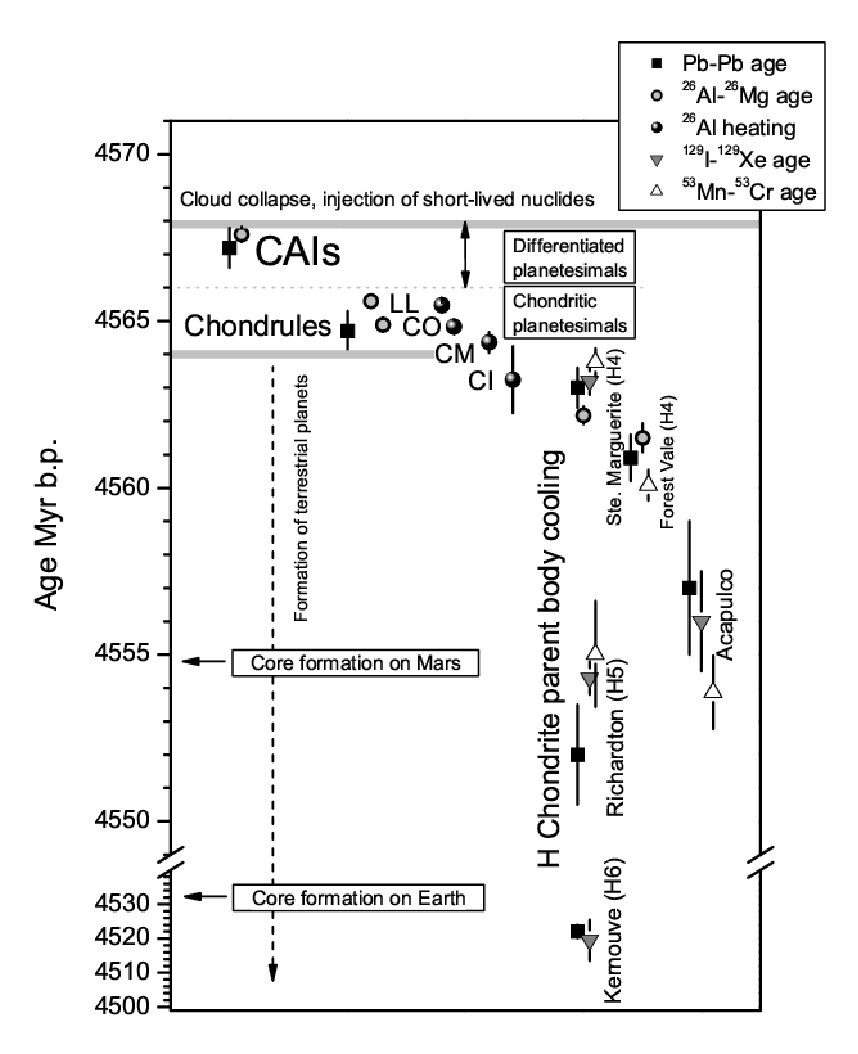
\includegraphics[width=8cm]{d1fig1.eps}}
\caption{Calibration of radioisotope time scales of early solar system
rocks: Pb-Pb (G\"opel et al.\ 1994; Amelin et al.\ 2002), Mn-Cr (Lugmair \&
Shukolyukov 1998, 2001; Polnau \& Lugmair 2001; Polnau et al.\ 2000), Al-Mg
(Zinner \& G\"opel 1992; Russell et al.\ 1996, 2001; Kita et al.\ 2000,
2004; Kunihiro et al.\ 2004), I-Xe (Nichols et al.\ 1994, Brazzle et al.\
1999). Red symbols are timescales according to planetesimal heating by
$^{26}$Al, from Trieloff and Palme (2006). }
\end{figure}

\subsection{Analysis of cometary matter returned by the STARDUST mission}

Comets have long been regarded as the chemically most primitive bodies in
our solar system, mostly due to their high abundance of volatiles: C, H, O,
N plus noble gases, at a level between solar and CI chondrite
composition. Particularly super-volatile species like CO demand that they
were stored most of their time at very low temperatures after
formation. However, IR spectroscopy of Hale-Bopp (Wooden et al.\ 2000)
already indicated that crystalline Mg-rich dust (forsterite, enstatite) is
present, an unexpected observation as these silicates are thought to be high
temperature products. Nevertheless this is in line with observations that
most of the sub-particles analyzed with NANO-SIMS in Interplanetary Dust Particles (IDPs) of presumably
cometary origin are isotopically solar (Messenger et al.\ 2003), and partly
have a high temperature origin, and also in line with one of the first
STARDUST results that CAI-like material was found among comet Wild-2
particles. As many scientists believe that these high temperature products
stem from the inner warm zones of our early solar system, these observations
have aroused strong interest in radial mixing processes of protoplanetary
discs, and in fact the observations place fundamental constraints on the
magnitude of these processes. The crucial number to be extracted from the
analysis of cometary dust is to identify and quantify the fraction of
material that experienced high temperature annealing, metamorphism,
condensation or evaporation and that was transported outwards subsequently. This
needs structural-chemical analysis, transmission electron microscopy (TEM),
and surface-sensitive Time-of-Flight Secondary Ion Mass Spectrometry
(TOF-SIMS). It is furthermore of importance to show that this material is
isotopically solar, i.e.\ equilibrated in the solar system, in order to
exclude the possibility that e.g.\ Mg-rich silicates are remnants of high
temperature condensation processes in the stellar envelope of a precursor
star nearby the cloud from which the solar nebula collapsed. This can only
be performed on sample returned material in the laboratory by NANO-SIMS
analysis. STARDUST (Brownlee et al.\ 1996) is the first extraterrestrial
sample return mission since the Apollo program, and the ongoing analysis can
provide such results, provided that systematic strategies are applied to
investigate keeping these goals in mind.


\section{Preliminary work (Eigene Vorarbeiten)}

M. Trieloff has broad experience in cosmochemistry and geochemistry,
particular the isotope radio-chronometry of processes in the early solar
system and their relationship to astrophysical processes in protoplanetary
disks. M. Trieloff conducted a number of studies on early meteorite
chronology and the accretionary and cooling history of meteorite parent
bodies (Trieloff et al.\ 2003; Kunz et al.\ 1995; Pellas et al.\ 1997;
Korochantseva et al.\ 2005). Combined $^{40}$Ar-$^{39}$Ar dating and $^{244}$Pu
fission track dating demonstrated that Acapulco and H4 chondrites Forest
Vale, St. Marguerite, and H5 Richardton are meteorites that formed early and
cooled rapidly in the high temperature (and partly also low temperature)
regime, i.e.\ that they recorded primary cooling histories and that later
secondary disturbances were insignificant.

M. Trieloff also studied processes that are related to the clearing of
accretions disk in the early solar nebula, leading to solar wind
implantation into precursor planetesimals of meteorite parent bodies and the
terrestrial planets (Trieloff et al.\ 2000, 2002; Trieloff and Kunz, 2005;
Schwarz et al.\ 2005). Trieloff and Palme (2006) reviewed and outlined the
early solar system history as seen by meteoriticists in the context of
astrophysical processes and disk evolution, specifically aimed at
astrophysically oriented scientists working on planet formation processes.

M. Trieloff has particular experience with $^{40}$Ar-$^{39}$Ar dating of
meteoritic matter (Trieloff et al.\ 2003; Kunz et al.\ 1995; Pellas et al.\
1997; Korochantseva et al.\ 2005) and implicitly the handling of neutron
irradiated samples as necessary for $^{129}$I-$^{129}$Xe
dating. $^{129}$I-$^{129}$Xe dating belongs to traditional noble gas studies
and was performed in Heidelberg previously (Jordan et al.\ 1980).

R. Altherr has broad expertise in the field of hard-rock petrology,
geochemistry and K-Ar geochronology. He has worked on the geodynamic
evolution of the Aegean, the Variscan belt of Central Europe and the Alps
including the formation of ultrahigh- and high-pressure metamorphic rocks
during subduction and continental collision (e.g.\ Altherr et al.\ 1979;
Schliestedt et al.\ 1988; Becker and Altherr, 1992; Kalt et al.\ 1995;
Altherr and Kalt, 1996; Kalt and Altherr, 1996; Paquin and Altherr,
2001). Another field of expertise are geochemical and petrographic studies
on high pressure and UHP mantle rocks (Paquin and Altherr, 2002, 2004;
Woodland et al.\ 2002; Olker et al.\ 2003; Witt-Eickschen et al.\ 2003).

The SIMS laboratory at the Mineralogical Institute has one of the few
national ion microprobes dedicated to geoscientific research. There
is experience with elemental and isotopic analysis of many elements, in
recent years focusing on Li, Be and B.

T. Stephan is member of four sub-teams of the STARDUST preliminary
examination team and correspondingly involved in the ongoing preliminary
examination phase for the STARDUST samples. There is considerable experience
in the analysis of cosmic dust (e.g.\ Stephan et al.\ 1994). In 1994,
T. Stephan initiated a still ongoing comprehensive consortium study of
particles from the stratospheric particle collector U2071 (Stephan et al.\
2001; Rost et al.\ 1998, 1999a, 1999b). In the last couple of years, IDP
research was focused on the identification of carriers of isotopic
anomalies, mainly 15N enrichments, in IDPs (Stephan and Stadermann, 2001;
Stephan, 2002; Stephan et al.\ 2003). This study in collaboration with the
Washington University in St. Louis brings together TOF-SIMS and NanoSIMS as
complementary techniques. Several IDPs from collector U2071 were
recently investigated at the Institute for Planetology in M\"unster and the
Max-Planck-Institute for Chemistry in Mainz (Hoppe et al.\ 2005; Stephan et
al.\ 2005). TEM in combination with TOF-SIMS and NanoSIMS allows a clear
structural identification of minerals that is not possible with the chemical
and isotopic information alone.  Together with established electron
microscope techniques (like SEM, TEM, and EMPA/electron microprobe analysis)
T. Stephan�s group uses especially TOF-SIMS for the analysis of small
grains. He introduced TOF-SIMS into the field of cosmochemistry and applied
this technique to the analysis of IDPs, presolar grains, and fine-grained
material in meteorites (e.g.\ Stephan 2001).



%
% Here follows the own refereed publications by the PIs in relation to
% the project proposed here.
%
\ownpubltitle{Own publications related to the Forschergruppe:}
%
% BELOW IS ONLY AN EXAMPLE OF TWO ENTRIES. SEE THE ADDITIONAL FILES 
% SENT TO YOU WITH ALL THE REFERENCES FROM THE VORANTRAG
%
\begin{ownpubl}
\item Altherr R. and Kalt A. (1996) Metamorphic evolution of ultrahigh-pressure garnet peridotites form the Variscan Vosges Mts. (France). Chem. Geol. \textbf{134}, 27-47.
\item Altherr R., Schliestedt M.,  Okrusch M., Seidel E., Kreuzer H., Harre W., Lenz H., Wendt I., Wagner G.A. (1979) Geochronology of high-pressure rocks on Sifnos (Cyclades, Greece). Contrib. Mineral.\ Petrol. \textbf{70}, 245-255.
\item Becker H. and Altherr R. (1992) Evidence from ultra-high-pressure marbles for recycling of sediments into the mantle. Nature \textbf{358}, 745-748.
\item Hoppe P., Mostefaoui S., and Stephan T. (2005) NanoSIMS oxygen- and
  sulfur-isotope imaging of primitive solar system materials. Lunar
  Planet. Sci. \textbf{36}, \# 1301 (abstr.).
\item Kalt A. and Altherr R. (1996) Metamorphic evolution of garnet-spinel peridotites from the Variscan Schwarzwald (Germany). Geol. Rundschau \textbf{85}, 211-224.
\item Kalt A., Altherr R., Hanel M. (1995) Contrasting P-T conditions recorded in ultramafic high-pressure rocks from the Variscan Schwarzwald (F.R.G.). Contrib. Mineral.\ Petrol. \textbf{121}, 45-60.
\item Korochantseva, E.V., Trieloff, M., Buikin, A.I., Meyer, H.P. and Hopp, J. (2005) Argon-40/Argon-39 dating, and cosmic ray exposure time of desert meteorites: Dhofar 300 and Dhofar 007 eucrites and anomalous achondrite NWA 011. \textit{Meteoritics and Planetary Science\/}, \textbf{40}, 1433
\item Kunz J., Trieloff M., Bobe K., Metzler K., St\"offler D., and Jessberger E.K. (1995) The collisional history of the HED parent body inferred from $^{40}$Ar-$^{39}$Ar ages of Eucrites. \textit{Planetary and Space Science\/}, \textbf{43}, 527-543.
\item Olker B, Altherr R, Paquin J (2003) Fast exhumation of the ultrahigh-pressure Alpe Arami garnet peridotite (Central Alps, Switzerland): constraints from geospeedometry and thermal modelling. Journal of Metamorphic Geology \textbf{21}, 395-402
\item Paquin J, Altherr R (2001) New constraints on the P-T evolution of the Alpe Arami garnet peritotide body (Central Alps, Switzerland). Journal of Petrology \textbf{42}, 1119-1140 
\item Paquin J, Altherr R (2002) Subduction-related lithium metasomatism during exhumation of the Alpe Arami ultrahigh-pressure garnet peridotite (Central Alps, Switzerland). Contributions to Mineralogy and Petrology \textbf{143}, 623-640 
\item Paquin J, Altherr R, Ludwig T (2004) Li-Be-B systematics in the ultrahigh-pressure garnet peridotite from Alpe Arami (Central Swiss Alps): implications for slab-to-mantle transfer. Earth and Planetary Science Letters \textbf{218}, 507-519 
\item Pellas, P., Fieni, C., Trieloff, M. and Jessberger, E.K. (1997) The cooling history of the Acapulco meteorite as recorded by the $^{244}$Pu and $^{40}$Ar-$^{39}$Ar chronometers. \textit{Geochimica et Cosmochimica Acta\/}, \textbf{61}, 3477
\item Rost D., Stephan T., and Jessberger E. K. (1999a) Surface analysis of stratospheric dust particles. Meteorit. Planet. Sci. \textbf{34}, 637�646. 
\item Rost D., Stephan T., Jessberger E. K., Nakamura K., and Kl\"ock W. (1998) New TOF-SIMS analyses of sections from stratospheric dust particles. Lunar Planet. Sci. \textbf{29}, \#1637 (abstr.).
\item Rost D., Stephan T., Wies C., and Jessberger E. K. (1999b) Analysis of sections and surfaces of inter-planetary dust particles. Meteorit. Planet. Sci. \textbf{34}, A99 (abstr.).
\item Schliestedt M., Altherr R., Matthews A. (1988) Evolution of the Cycladic crystalline complex: petrology, isotope geochemistry and geochronology. In: H. C. Helgeson (Editor), Chemical Transport in Metasomatic Processes. NATO-ASI Series, Reidel, Dordrecht, pp. 389-428.
\item Schwarz W.H., Trieloff M. and Altherr R. (2005) Subduction of solar type noble gases from extraterrestrial dust: Constraints from high-pressure low-temperature metamorphic deep sea sediments. \textit{Contributions to Mineralogy and Petrology\/}, \textbf{149}, 675-684.
\item Stephan T. (2001) TOF-SIMS in cosmochemistry. Planet. Space Sci. \textbf{49}, 859�906. 
\item Stephan T. (2002) TOF-SIMS analysis of heavy-nitrogen-carrying phases in interplanetary dust. Lunar Planet. Sci. \textbf{33}, \#1352 (abstr.). 
\item Stephan T. and Stadermann F. J. (2001) Preliminary identification of a heavy-nitrogen-carrying phase in IDPs. Meteorit. Planet. Sci. \textbf{36}, A197�A198 (abstr.). 
\item Stephan T., Arndt P., Jessberger E. K., Kl\"ock W., Nakamura K., Maetz M., Rost D., Thomas-Keprta K. L., Warren J. L., Weber I., and Wies C. (2001) Comprehensive consortium study of interplanetary dust particles from collector U2071. Lunar Planet. Sci. \textbf{32}, \#1267 (abstr.). 
\item Stephan T., Jessberger E. K., Kl\"ock W., Rulle H., and Zehnpfenning J. (1994) TOF-SIMS analysis of interplanetary dust. Earth Planet. Sci. Lett. \textbf{128}, 453�467. 
\item Stephan T., Leitner J., Floss C., and Stadermann F. J. (2003) TOF-SIMS analysis of isotopically anomalous phases in interplanetary dust and Renazzo. Lunar Planet. Sci. \textbf{34}, \#1343 (abstr.). 
\item Stephan T., Weber I., and Hoppe P. (2005) TOF-SIMS, NanoSIMS, and TEM analysis of interplanetary dust particle sections. Lunar Planet. Sci. \textbf{36}, \#1645 (abstr.).
\item Trieloff, M. and Kunz, J. (2005) Isotope systematics of noble gases in the Earth�s mantle: Possible sources of primordial isotopes and implications for mantle structure. \textit{Physics of the Earth and Planetary Interiors\/}, \textbf{148}, 13
\item Trieloff, M. and Palme, H. (2006) The origin of solids in the early solar system. In: \textit{Planet Formation - Theory, Observations, and Experiments}. (Eds. H. Klahr, W. Brandner), Cambridge University Press, Cambridge, 64
\item Trieloff, M., Falter, M., Buikin, A.I., Korochantseva, E.V., Jessberger, E.K. and Altherr R. (2005) Argon isotope fractionation induced by stepwise heating. \textit{Geochimica et Cosmochimica Acta\/}, \textbf{69}, 1253
\item Trieloff, M., Jessberger, E.K., Herrwerth, I., Hopp, J., Fi�ni, C., Gh�lis, M., Bourot-Denise, M. and Pellas, P. (2003) 244Pu and 40Ar-39Ar thermochronometries reveal structure and thermal history of the H-chondrite parent asteroid. \textit{Nature\/}, \textbf{422}, 502
\item Trieloff, M., Kunz, J. and All�gre, C.J. (2002) Noble gas systematics of the R�union mantle plume source and the origin of primordial noble gases in Earth�s mantle. \textit{Earth and Planetary Science Letters\/}, \textbf{200}, 297
\item Trieloff, M., Kunz, J., Clague, D.A., Harrison, D. and All�gre, C.J. (2000) The nature of pristine noble gases in mantle plumes. \textit{Science\/}, \textbf{288}, 1036
\item Witt-Eickschen G, Seck HA, Mezger K, Eggins SM, Altherr R (2003) Lithospheric mantle evolution beneath the Eifel (Germany): constraints from Sr-Nd-Pb isotopes and trace element abundances in spinel peridotite and pyroxenite xenoliths. Journal of Petrology \textbf{44}, 1077-1095 
\item Woodland AB, Seitz H-M, Altherr R, Marschall H, Olker B, Ludwig T (2002) Li abundances in eclogite minerals: a clue to a crustal or mantle origin? Contributions to Mineralogy and Petrology \textbf{143}, 587-601
\end{ownpubl}
%



\section{Goals (Ziele)}
\begin{enumerate}
\item Isotope chronology of chondrule populations
\begin{compactitemize}
\item Determine age constraints for planetesimal formation by applying I-Xe and
  $^{26}$Al-$^{26}$Mg chronometry to chondrules. Check age distributions of
  chondrule populations of single meteorites and differences between age
  distributions of meteorites from different classes, mainly between
  ordinary and carbonaceous chondrites.
\item Constrain models of timing of planetesimal growth in the early solar
  system, i.e.\ duration of accretion of single parent bodies, sequence of
  accretion of different parent bodies: how many Myr after CAIs did
  individual parent bodies accrete, how long did they need for accretion,
  and what was the age of the accreted precursor chondrules?
\end{compactitemize}
\item Analysis of cometary matter returned by the STARDUST mission
\begin{compactitemize}
\item Quantify the proportion of high temperature products (thermally
annealed crystalline material, high temperature condensates or evaporation
residues). Constrain fraction of the material that originated from the inner
disk and were transported into the outer disc regions where comets
formed. While TEM and TOF-SIMS analyses will allow to infer the
structural-mineralogical-chemical state of cometary dust (amorphous,
crystalline, chemical composition), NANO-SIMS studies will further quantify
the fraction of unprocessed interstellar dust and dust components processed
in the early solar system. These numbers constrain radial mixing processes
to the outer disk, and are needed in project A2.
\end{compactitemize}
\end{enumerate}



\section{Work schedule (Arbeitsprogramm)}

(this section only refers to goal Isotope chronology of chondrule
populations. STARDUST analyses are described and performed in a separate DFG
proposal, code no. STE 576/17

\subsection{Methods}
The basic strategy will be to use two different short-lived nuclide systems
($^{129}$I-$^{129}$Xe, $^{26}$Al-$^{26}$Mg) in order to check age
distributions that previously relied on one single chronometer. For this
study the Heidelberg Mineralogical institute has experienced laboratory
facilities. Different diffusion parameters of daughter nuclides in relevant
host minerals (Mg, Xe) should allow to distinguish artifacts, e.g.\ if shock
or thermally induced (partial or complete) reset of radiometric systems
causes irrelevant low ages, or if incomplete reset of the radiometric clock
during formation causes irrelevant high ages. For I-Xe dating of chondrules,
improvements could be achieved by a more comprehensive identification of
host phases carrying iodine. Such phases can be searched for in individual
chondrules using combined electron and ion microprobe studies. Iodine should
be enriched in the mesostasis, but pyroxene is a potential carrier as well
(Pravdivtseva et al.\ 1998). It may also be feasible to identify (and remove
by mineral separation or etching) iodine phases of low xenon retentivity in
order to avoid phases disturbed by secondary events.

Chondrules will be separated from selected meteorites from different
chondrite classes. Meteorites must be chosen in which the radiometric
systems are not or not recognizably disturbed by processes following
chondrule formation (thermal or aqueous metamorphism on the parent body,
impact/shock induced reheating). Ar-Ar data from an unpublished doctoral
thesis in Heidelberg (Herrwerth, 1983), and other I-Xe and
$^{26}$Al-$^{26}$Mg studies will help to select appropriate
samples. Chondrites with an obvious undisturbed I-Xe system of chondrules
are L4 Bjurb\"ole and - possibly - CV3 Allende (see compilation by Whitby,
2004). L4 Saratov and H4 Ochansk have easily separable chondrules with
undisturbed K-Ar systems (Herrwerth 1983). CO 3.0 Y81020 and the H
chondrites H3 Tieschitz, H4s Forest Vale, Ste. Marguerite, Beaver Creek,
Ankober, Quenggouk are worthwhile to be checked based on their low
processing degree established by $^{26}$Al-$^{26}$Mg, $^{40}$Ar-$^{39}$Ar
and $^{244}$Pu fission track studies (Kunihiro et al.\ 2004; Zinner \&
G\"opel. 1992; Trieloff et al.\ 2003). Some LL3 chondrites (e.g.\ 3.4
Chainpur, 3.6 Parnallee) are disturbed in their Ar-Ar and I-Xe systems
(Herrwerth 1983; Whitby 2004). Part of the chondrules from 3.0 Semarkona
seem also disturbed in the I-Xe system (Whitby 2004), while the Al-Mg system
of most chondrules from this meteorite seems to record primary formation
events (Kita et al.\ 2000, 2004). Further studies on LL3.1 Bishunpur can
supplement the study, and other promising meteorite samples will be searched
on in the course of the study.

We are - of course - aware of the problem that parent body metamorphism
(reflected in petrologic type) may have reset radiometric systems. However,
the fact that 3.4 or 3.6 LL chondrites (Chainpur, Parnallee) are disturbed,
may not imply that stronger metamorphosed type 4 chondrites were disturbed
or reset as well. In the case of Chainpur, Ar-Ar ages indicate that
disturbances happened a few 100 Ma after thermal metamorphism (Herrwerth,
1983). Hence, not parent body metamorphism itself (reflected in the subtype
3.4 classification) was the likely cause of disturbance, but probably
secondary impact metamorphism induced by a collisional event. Bjurb\"ole,
although of petrologic type 4, has whole rock ages well up to 2-4 Ma older
than Shallowater enstatite (Brazzle et al.\ 1999; Gilmour et al.\ 2006),
well within the range of earliest chondrule ages (Gilmour et al.\ 2006), so
a reset of the clock by parent body metamorphism is not evident, at least
not obvious. On the other hand, the I-Xe and Al-Mg system of H4
Ste. Marguerite feldspar (this secondary mineral phase formed upon thermal
parent body metamorphism) seems to have recorded a post chondrule formation
event, most likely (rapid) cooling due to parent body metamorphism. In this
context it is important to note that the petrologic type 4 classification (a
discrete classification scheme) encompasses a wide range of maximum
metamorphic temperatures ranging from 600�C-700�C. This is also reflected by
the varying integration degrees of chondrules and matrix, and implies the
possibility that the degree of disturbance of specific meteorites and their
mineral phases could have been very different, and does not exclude type 4
chondrites as possible sample for the studies suggested here.

From each ordinary chondrite / carbonaceous chondrite sample, 10-20
chondrules will be separated. While the larger parts of them will be kept
for possible I-Xe analysis, a smaller part will be sectioned and classified
by optical and electron microscopy. Electron microprobe analysis will
further help to classify chondrules, establish mineralogical/petrographic
properties and enable subsequent ion microprobe studies. Preliminary ion
microprobe inspections will allow the recognition of $^{26}$Mg excess, and
possible iodine carrier phases in chondrules (mesostasis, pyroxene, etc),
including their iodine concentrations, in order to select the most promising
samples for I-Xe analysis.

I-Xe analysis of single chondrules with phases enriched in iodine (of
different chondrite types) and the possible use of cumulate samples of type
I, type II chondrules will lead to an increased precision. Moreover, the use
of mineral separates (e.g.\ pyroxene) seems advisable to get a better
control of carrier phases, closure temperatures and comparability of
results/I-Xe ages. Particularly pyroxene is a more retentive carrier for
argon (as monitored by neutron induced $^{37}$Ar, e.g.\ Trieloff et al.\
2003) and hence a promising candidate for a retentive, undisturbed host
phase of radiogenic $^{129}$Xe. Separates of the Shallowater I-Xe standard
shall be used throughout the project; we will additionally check the
homogeneity of the Iodine distribution via SIMS.

For samples successfully dated with I-Xe, ion microprobe investigations can
� if not succeeded during the preliminary investigation - constrain
iodine carrier phases (especially in the light of degassing reservoirs
identified during Xe analyses), and will perform $^{26}$Al-$^{26}$Mg dating
of individual chondrules. Comparison of these data will allow to check for
age differences within chondrule populations (e.g.\ possibly dependent on
chondrule chemistry), and to quantify age distributions. The ultimate goal
is to compare the age distributions between different meteorite classes. The
most favorable case would be to obtain consistent results of the two
chronometric systems, but also inconsistent results can yield valuable
information: they could indicate that the different chronometers date
different events, or were incompletely reset or responded differently to
subsequent disturbances. Just as an example, if I-Xe does not reproduce
older chondrule ages from $^{26}$Al-$^{26}$Mg, this could mean that the
$^{26}$Al-$^{26}$Mg was not completely reset during chondrule formation,
i.e.\ that high chondrule ages are not formation ages.

Personal support and laboratory equipment in Heidelberg for mineral
separation and chondrule preparation, SEM and electron microprobe analytical
facilities, noble gas mass spectrometer for analysis of neutron irradiated
samples, ion microprobe is available. The noble gas lab in Heidelberg is one
of the few worldwide (and only one in Germany) engaged in dating with noble
gas nuclides of neutron irradiated extraterrestrial samples, and has
significant expertise in this field (e.g.\ Trieloff et al.\ 2003; Kunz et
al.\ 1995; Pellas et al.\ 1997; Korochantseva et al.\ 2005). In addition to
Ar-Ar dating, I-Xe dating can be performed with the same technique (neutron
irradiated samples, noble gas isotope analysis), but yields a better time
resolution/precision for early solar system processes. Moreover, Heidelberg
has one of the few ion microprobes used for geological/extraterrestrial
samples. The ion microprobe analytic facility has been repeatedly improved
by in-house constructional efforts. Ion microprobe analyses are the standard
technique for $^{26}$Al-$^{26}$Mg dating.


\subsection{Schedule}
\subsubsection{First year}

Preparation of chondrule separates of various ordinary and carbonaceous
chondrites (if appropriate mineral separations) and I-Xe dating
standards. Mineralogical/petrographic characterization of chondrule thin
sections (Optical, SEM, EMPA), and first SIMS analyses. Irradiation and
first xenon isotope dating.

\subsubsection{Second year}

Continuation of xenon isotope dating, EMPA analyses and Mg isotope
measurements with ion microprobe.

\subsubsection{Third year}

Final experiments/analyses, preparation of thesis and publications


\subsection{Literature}
%
% Here follows a general literature list related to the topic of the
% proposal, just like a literature list for a scientific paper.
%
% AGAIN ONLY EXAMPLES ARE LISTED NOW
%
\begin{literature}
\item All\`egre, C.J., Manh\`es, G., and G\"opel C. (1995).  The age of the Earth, \textit{Geochim. Cosmochim. Acta} \textbf{59}, 1445--1456.   
\item Amelin Y., Krot A. N., Hutcheon I.D. and Ulyanov A.A. (2002).  Lead isotopic ages of chondrules and calcium-aluminum-rich inclusions.  \textit{Science} \textbf{297}, 1678--1682.   
\item Amelin Y. (2006) The prospect of high precision Pb isotopic dating of meteorites. \textit{Met. Planet. Sci.} 41, 7-17.
\item Birck, J.-L. and All\`egre, C. J. (1985).  Evidence for the presence of $^{53}$Mn in the early Solar System, \textit{Geophys. Res. Lett.} \textbf{12}, 745--748.
\item Bizzarro, M., Baker, J. A. and Haack, H. (2004).  Mg isotope evidence for contemporaneous formation of chondrules and refractory inclusions, \textit{Nature} \textbf{431}, 275--278.
\item Bockel\'ee-Morvan, D., Gautier, D., Hersant, F., Hur\'e, J.M., and Robert, F. (2002) Turbulent radial mixing in the solar nebula as the source of crystalline silicates in comets. \textit{Astronomy and Astrophysics\/}, \textbf{384}, 1107
\item Boss A.P. and Vanhala H.A.T. (2001).  Injection of newly synthesized elements into the protosolar cloud, \textit{Phil. Trans. R. Soc. Lond.} \textbf{A 359}, 2005--2017.   
\item Brazzle R.H., Pravdivtseva O.V., Meshik A.P. and Hohenberg C.M. (1999).  Verification and interpretation of the I-Xe chronometer.  \textit{Geochim. Cosmochim Acta} \textbf{63}, 739--760.   
\item Brownlee D. E., Burnett D. {\em et~al.} (1996).  Stardust: Comet and interstellar dust sample return mission, in \textit{Physics, Chemistry, and Dynamics of Interplanetary Dust}, ed. B.A.S.~Gustafson and M.S.~Hanner (ASP Conf. Series 104).   
\item Chen J.H. and Wasserburg G.J. (1981).  The isotopic composition of uranium and lead in Allende inclusions and meteoritic phosphates.  \textit{Earth Planet. Sci. Lett.} \textbf{5}, 15--21.   
\item Desch, S. J. and Connolly Jr., H. C. (2002).  A model of the thermal processing of particles in solar nebula shocks: application to the cooling rates of chondrules.  \textit{Meteoritics and Planetary Science} \textbf{37}, 183.   
\item Dodd R. T. (1969).  Metamorphism of the ordinary chondrites: A review.  \textit{Geochim. Cosmochim. Acta} \textbf{33}, 161--203.   
\item Gail, H.-P. (2003).  Formation and evolution of minerals in accretion disks and stellar outflows, in \textit{Astromineralogy }, ed. T.K.~Henning (Springer, Heidelberg).   
\item Gail, H.-P. (2004).  Radial mixing in protoplanetary accretion disks IV. Metamorphosis of the silicate dust complex.  \textit{Astron. Astrophys.} \textbf{413}, 571--591.   
\item Gilmour J.D., Pravdivtseva O.V., Busfield A., and Hohenberg C.M. (2004).  I-Xe and the chronology of the early solar system.  \textit{Workshop on chondrites and the protoplanetary disk} abstr. no. 9054.
\item Gilmour J.D., Pravdivtseva O.V., Busfield A., and Hohenberg C.M. (2006).  The I-Xe chronometer and the early solar system.  \textit{Met. Planet. Sci.} 41, 19-31.
\item Gilmour J.D. and Saxton, J.M. (2001).  A time-scale of formation of the first solids, \textit{Phil. Trans. R. Soc. Lond.} \textbf{A 359}, 2037--2048.   
\item G\"opel C., Manh\`es G., and All\`egre C.J. (1994).  U-Pb systematics of phosphates from equilibrated ordinary chondrites.  \textit{Earth Planet. Sci. Lett.} \textbf{121}, 153--171.   
\item Halliday A.N., Lee D-C. {\em et~al.} (2001).  The rates of accretion, core formation and volatile loss in the early Solar System.  \textit{Phil. Trans. R. Soc. Lond.} \textbf{A 359}, 2095.   
\item Hartmann L. (2001).  Physical conditions of protosolar matter.  \textit{Phil. Trans. R. Soc. Lond.} \textbf{A 359}, 2049--2060.
\item Herrwerth I., M\"uller N., Jessberger E.K., Kirsten T. (1983) $^{40}$Ar-$^{39}$Ar Dating of Individual Chondrules and the Siting of Trapped Argon. Met. 18, 311.
\item Jeffery P.M. and Reynolds J.H. (1961).  Origin of excess Xe$^{129}$ in stone meteorites.  \textit{J. Geophys. Res.} \textbf{66}, 3582--3583.   
\item Jordan, J.; Kirsten, T.; Richter, H. (1980) I-129/I-127 - A puzzling early solar system chronometer. Z. Naturforschung 35 a, 145-170.
\item Kita N.T., Nagahara H., Togashi S. and Morishita Y. (2000).  A short duration of chondrule formation in the solar nebula: Evidence from Al-26 in Semarkona ferromagnesian chondrules \textit{Geochim. Cosmochim. Acta} \textbf{64}, 3913--3922.
\item Kita N.T., Huss G.R. {\em et~al.} (2004).  Constraints on the origin of chondrules and CAIs from short-lived and long-lived radionuclides.  \textit{Workshop on chondrites and the protoplanetary disk, abstr. no \#9064.}   
\item Kleine, T., M\"unker, C. {\em et~al.} (2002).  Rapid accretion and early core formation on asteroids and the terrestrial planets from Hf-W chronometry.  \textit{Nature} \textbf{418}, 952.
\item Kleine, T., Mezger, K., Palme, H., Scherer, E. and M\"unker, C. (2005).  Early core formation in asteroids and late accretion of chondrite parent bodies: Evidence from 182Hf-182W in CAIs, metal-rich chondrites and iron meteorites.  \textit{Geochim. Cosmochim. Acta}, \textbf{69}, 5805
\item Klerner S. and Palme H. (2000).  Formation of chondrules and matrix in carbonaceous chondrites.  \textit{Met. Plan. Sci.} \textbf{35}, A89.   
\item Kn\"odlseder J., Cervino M., Le Duigou J.M., Meynet G., Schaerer D. and von Ballmoos P. (2002).  Gamma-ray line emission from OB associations and young open clusters - II. The Cygnus region.  \textit{Astron. Astrophys.} \textbf{390}, 945--960.   
\item Kokubo, E. and Ida, S. (2000).  Formation of protoplanets from planetesimals in the solar nebula.  \textit{Icarus} \textbf{143}, 15. 
\item Kunihiro T., Rubin A.E., McKeegan K.D. and Wasson J.T. (2004).  Initial $^{26}$Al/$^{27}$Al in carbonaceous-chondrite chondrules: Too little $^{26}$Al to melt asteroids.  \textit{Geochim. Cosmochim. Acta} \textbf{68}, 2947--2957.    
\item Kurahashi, E.; Kita, N. T.; Nagahara, H.; Morishita, Y. (2004) Contemporaneous Formation of Chondrules in the $^{26}$Al-$^{26}$Mg System for Ordinary and CO Chondrites. Lun. Planet. Sci. XXXV, abstract no.1476
\item LaTourrette T. and Wasserburg G.J. (1998).  Mg diffusion in anorthite: implications for the formation of early solar system planetesimals.  \textit{Earth Planet. Sci. Lett.} \textbf{158}, 91--108.   
\item Lee T., Papanastassiou D.A. and Wasserburg G.J. (1976).  Demonstration of $^{26}$Mg excess in Allende and evidence for $^{26}$Al.  \textit{Geophys. Res. Lett.} \textbf{3},109--112.   
\item Lee, T., Shu, F. H. {\em et~al.} (1998).  Protostellar cosmic rays and extinct radioactivities in meteorites.  \textit{Astrophys. J.} \textbf{506}, 898.   
\item Lugmair, G.W. and Shukolyukov, A. (2001).  Early solar system events and time scales.  \textit{Met. Planet. Sci.} \textbf{36}, 1017.   
\item Lugmair G.W. and Shukolyukov A. (1998).  Early solar system timescales according to 53 Mn-53 Cr systematics.  \textit{Geochim. Cosmochim. Acta} \textbf{62}, 2863--2886.    
\item McKeegan, K. D., Chaussidon, M. and Robert, F. (2000).  Incorporation of short-lived $^{10}$Be in a calcium-aluminum-rich inclusion from the Allende meteorite.  \textit{Science} \textbf{289}, 1334--1337.   
\item Messenger, S., Keller, L. P. {\em et~al.} (2003).  Samples of stars beyond the solar system: Silicate grains in interplanetary dust.  \textit{Science} \textbf{300}, 105.   
\item Mostefaoui, S. Kita N.~T. et al. (2002)[ The relative formation ages of ferromagnesian chondrules inferred from their initial aluminum-26/aluminum-27 ratios.] Met. Planet. Sci., 37, 421.
\item Nichols, R. H., Jr.; Hohenberg, C. M.; Kehm, K, Kim Y., Marti K. (1994) I-Xe studies of the Acapulco meteorite: Absolute I-Xe ages of individual phosphate grains and the Bjurb\"ole standard. Geochim. Cosmochim Acta 58, 2553-2561.
\item Palme, H. (2001).  Chemical and isotopic heterogeneity in protosolar matter.  \textit{Phil. Trans. R. Soc. Lond.} \textbf{A 359}, 2061.   
\item Pellas P., Fieni C., Trieloff M. and Jessberger, E.K. (1997).  The cooling history of the Acapulco meteorite as recorded by the $^{244}$Pu and $^{40}$Ar-$^{39}$Ar chronometers.  \textit{Geochim. Cosmochim. Acta} \textbf{61}, 3477--3501.    
\item Polnau E. and Lugmair G.W. (2001).  Mn-Cr isotope systematics in the two ordinary chondrites Richardton (H5) and Ste. Marguerite (H4).  \textit{Lun. Planet. Sci. XXXII, abstr. no \#1527}.
\item Polnau, E.; Lugmair, G. W.; Shukolyukov, A.; MacIsaac, Ch (2000) Manganese-Chromium-Isotopic Systematics in the Ordinary Chondrite Forest Vale (H4). Meteoritics \& Planetary Science, 35, A128
\item Russell S.S., Srinivasan G., Huss G.R., Wasserburg, G.J. and MacPherson G.J. (1996).  Evidence for widespread $^{26}$Al in the solar nebula and constraints for nebula time scales.  \textit{Science} \textbf{273}, 757--762.  
\item Russell S.S., Gounelle M. and Hutchison R. (2001).  Origin of short-lived radionuclides \textit{Phil. Trans. R. Soc. Lond.} \textbf{A 359}, 1991.    
\item Scott E.R.D., Love S.G. and Krot A.N. (1996) Formation of chondrules and chondrites in the protoplanetary nebula, in \textit{Chondrules and the protoplanetary disk}, ed. R.H.~Hewins, R.H. ~Jones and E.R.D.~Scott (Cambridge University Press).   
\item Sears D.W.G. and Dodd R.T. (1988) Overview and classification of meteorites, in \textit{Meteorites and the early solar system}, ed. J.F.~Kerridge and M.S.~Matthews (University of Arizona Press, Tucson).   
\item Sears, D.W.G. (2004).  \textit{The origin of chondrules and chondrites} (Cambridge University Press).   
\item Shu F. H., Shang H. and Lee T. (1996).  Toward an astrophysical theory of chondrites.  \textit{Science} \textbf{271}, 1545--1552.    
\item Shukolyukov A. and Lugmair G. W. (1993) Life iron-60 in the early solar system.  \textit{Science} \textbf{259}, 1138--1142.   
\item Swindle and Podosek (1988). Iodine-xenon dating in: Meteorites and the early solar system, ed. Kerridge J.F. \& Matthews M.S. pp. 1127-1146. University of Arizona Press, Tucson, Arizona.
\item Tachibana S. and Huss G.R. (2003).  The initial abundance of Fe-60 in the solar system.  \textit{Astrophys. J.} \textbf{588}, L41--L44.   
\item Trieloff, M., Kunz, J. {\em et~al.} (2000).  The nature of pristine noble gases in mantle plumes.  \textit{Science} \textbf{288}, 1036--1038.   
\item Trieloff M., Kunz J. and All\`egre C.J. (2002).  Noble gas systematics of the R\'eunion mantle plume source and the origin of primordial noble gases in Earth�s mantle.  \textit{Earth Planet. Sci. Lett.} \textbf{200}, 297--313.   
\item Trieloff M., Jessberger E.K., Herrwerth I., Hopp J., Fieni C., Ghelis M., Bourot-Denise M. and Pellas P. (2003).  $^{244}$Pu and $^{40}$Ar-$^{39}$Ar thermochronometries reveal structure and thermal history of the H-chondrite parent asteroid.  \textit{Nature} \textbf{422}, 502--506.   
\item Turner G., Enright M.C. and Cadogan P. H. (1978).  The early history of chondrite parent bodies inferred from $^{40}$Ar-$^{39}$Ar ages.  \textit{Proc. Lunar Planet. Sci. Conf.} \textbf{9th}, 989--1025.    
\item van Schmus W.R. and Wood J.A. (1967).  A chemical-petrologic classification for the chondritic meteorites.  \textit{Geochim. Cosmochim. Acta} \textbf{31}, 747--765.    
\item Wasserburg, G. J., Gallino, R., and Busso, M. (1998).  \textit{Astrophys. J.} \textbf{500}, L189.    
\item Wetherill, G. W. and Stewart, G. R. (1993).  Formation of planetary embryos: Effects of fragmentation, low relative velocity, and independent variation of eccentricity and inclination.  \textit{Icarus} \textbf{106}, 190.
\item Whitby, J.A. (2004) Over What Period of Time Did Chondrule Formation Occur? \textit{Workshop on chondrites and the protoplanetary disk} abstr. no. 9101.
\item Wooden D. H., Butner, H. M. {\em et~al.} (2000).  Mg-rich silicate crystals in comet Hale-Bopp: ISM relics or solar nebula condensates?  \textit{Icarus} \textbf{43}, 126.   
\item Zinner E. and G\"opel C. (2002).  Aluminum-26 in H4 chondrites: Implications for its production and its usefulness as a fine-scale chronometer for early solar system events.  \textit{Met. Planet. Sci.} \textbf{37}, 1001--1013.   
%
%\item {\bf **************** PUT STUFF INTO ALPH ORDER ******************}
\end{literature}



\section{External/International collaborations}
\subsection{Isotope chronology of chondrule populations, Institute of Mineralogy, Heidelberg.}
\begin{collablist}
\item[Washington University, St.~Louis] O.V.~Pravdivtseva, A.P.~Meshick: leading experts in
I-Xe dating, advisory team and cooperation measurements for I-Xe dating. 
\end{collablist}

\subsection{Analyses of cometary matter returned by the STARDUST mission, Institute of Planetology, M\"unster}

Intense contacts between the Institute of Planetology (M\"unster) and other
scientists investigating Stardust samples exist, especially to Prof. D. E. Brownlee (University of Washington, Seattle), Prof. G. J. Flynn (State University of New York, Plattsburgh), 
Dr. M. E. Zolensky and Dr. F. H�rz (NASA Johnson Space Center, Houston), 
Dr. Scott Sandford (NASA Ames Research Center, Moffett Field), Dr. J. P. Bradley 
(Lawrence Livermore National Laboratory). For the investigation of presolar grains from
Meteorites and IDPs, we cooperate with Prof. E. K. Zinner and Dr. S. Amari (both
Washington University, St. Louis) as well as Priv.-Doz. P. Hoppe. Especially
with Dr. Hoppe (Mainz) and Dr. Stadermann we plan to extend the joint effort to investigate
presolar phases in IDPs and the STARDUST samples. The NanoSIMS
instruments present in Mainz and St. Louis will be of great importance in this
context. In analytics, close cooperation exists
with Prof. H. Arlinghaus (Physikalisches Institut, M\"unster) as well as
Dr. E. P. Vicenzi and Dr. D. Rost (Smithsonian Institute, Washington) on
TOF-SIMS and Prof. A. Putnis (Institut f\"ur Mineralogie, M\"unster) on TEM.



\section{Link to other projects of the Forschergruppe}
  
%\begin{linkproj}
%\item[\projdul{},\projklahr{},\projtscharn{}] Data will improve the timing
%of the process of planetesimal accretion in the early solar system, and
%accordingly provides constraints on models of planetesimal growth in
%projects \projdul{}, \projklahr{}, and \projtscharn{}.
%\item[\projwolf{}] As timing of accretion/coagulation also significantly
%influences the distribution of primary dust, the project will provide
%constraints for future observations of protoplanetary disks aimed in project
%\projwolf{}. {\bf SUGGESTION BY KEES TO MARIO: Perhaps also relate to the
%measured ages of the stars, even though this is sometimes a bit
%uncertain}. Similarly, the presence of planetesimals with minerals produced
%by hydrothermal alteration processes will indicate planetesimals via the
%presence of secondary, impact induced debris dust consisting of hydrous
%silicates.
%\end{linkproj}

\begin{linkproj}
\item[C1,C2,A2] The new Isotope chronology data will improve and refine the timing of the
process of planetesimal accretion in the early solar system, and accordingly
provides constraints on models of planetesimal growth in accretion disk
models by C. Dullemond/T. Henning (C2), H. Klahr/W. Kley (C1), and
W.M. Tscharnuter/H.-P. Gail/ T. Henning (A2). 

\item[D2] As timing of accretion/coagulation also significantly influences the
distribution of primary dust, the project will provide constraints for
future observations of protoplanetary disks aimed in the project by S. Wolf
(D2). For example, the presence of planetesimals with minerals produced by
hydrothermal alteration processes will indicate planetesimals via the
presence of secondary, impact induced debris dust consisting of hydrous
silicates.

\item[A1,A2] Data obtained by STARDUST analyses will provide important constraints for
project A2 (occurrence of annealed silicates or refractory condensates in
comet formation regions). Formation conditions of such high temperature
products can be checked by experimental work to be done in A1. 

\item[B1,B2,B3] Primary
accretional textures found in cometary dust can provide important hints of
coagulation processes studied by B1, B2, B3. The chemistry and texture of
chondrites as well gives a snapshot of syn-accretional conditions. This
snapshot can be compared with the outcome of collisional experiments in
Block B, e.g. if highly porous aggregates were direct precursors before
chondrite compaction, and if chondrules or their formation processes played
a role in speeding up the planetesimal formation process.

\end{linkproj}



\section{Team members (Zusammensetzung der Arbeitsgruppe)}
%
% NOTE: Only list non-DFG-funded team members.
% NOTE: Also list technical assistants, students etc involved in the project
%
\subsection{`Isotope chronology of chondrule populations�, Institute of
  Mineralogy, Heidelberg}
\begin{teamlist}
\item[Trieloff, M., Dr. Priv. Doz.]\mbox{}\\
Team leader of noble gas isotope geochronology group.  Supervision of PhD
student, particular I-Xe measurements, integration of results and early
solar system chronology, transfer to projects A2, B1, B2, B3, C2, D2.
\item[Prof. Dr. R. Altherr, head of Mineralogical Institute]\mbox{}\\
Supervision of electron and ion microprobe measurements.
\item[Dr. H.P.-Meyer]\mbox{}\\
Electron microprobe laboratory, Mineralogical Institute: Assistance in
electron microprobe analyses.
\item[Dipl. Phys. Th. Ludwig]\mbox{}\\
Secondary Ion microprobe laboratory, Mineralogical Institute: Assistance in
ion microprobe analyses.
\item[Dr. W. Schwarz (DFG)]\mbox{}\\
Noble gas mass spectrometry laboratory, Mineralogical Institute: Assistance
in I-Xe dating experiments, noble gas mass spectrometry
\item[Dr. J. Hopp (DFG)]\mbox{}\\
Noble gas mass spectrometry laboratory, Mineralogical Institute: Assistance
in I-Xe dating experiments, noble gas mass spectrometry
\end{teamlist}
%\vspace{1em}

\subsection{`Analyses of cometary matter returned by the STARDUST mission�, 
   Institute of Planetology, M\"unster}
\begin{teamlist}
\item[HDoz. Dr. T. Stephan]\mbox{}\\
(applicant of DFG project code no. STE 576/17)
\item[Prof. Dr. E. K. Jessberger]\mbox{}\\
(applicant of DFG project code no. STE 576/17)
\item[Dipl. Phys. Jan Leitner]\mbox{}\\
(PhD student within DFG project code no. STE 576/17)
\item[N.N.]\mbox{}\\
(TEM specialist within  DFG project code no. STE 576/17)
\item[CTA Kerstin Klemm]\mbox{}\\
\end{teamlist}



\section{Funding requested}
The following table gives the full overview of requested
funding:\vspace{1\baselineskip}\\

(this section refers to `Isotope chronology of chondrule populations� only, 
the STARDUST project is funded by a separate ongoing DFG project, 
proposal code no. STE 576/17 � except for 4 travels Heidelberg-M�nster 
are applied here for collaboration STARDUST-Forschergruppe)

%
% The table that follows is the overview over the full requested 
% funding, including the positions, travel, consumables and ``other
% costs'' (which might include transportation costs of radioactive
% material or the rent of a drop tower or such).
%
\centerline{\begin{tabular}{||l|l|l|l||} \hline \hline & Year 1 & Year 2 &
Year 3 \\ \hline %
Personel (1 PhD-student: E13/2)   & \hfil 24.000 & 24.000 & 24.000 \\
Personnel (1 student research assistant (30 hours/month) & \hfil 4.500 & \hfil 2.250 & \hfil - \\
Consumables                        & \hfil 8.300 & \hfil 8.300 & \hfil 4.800 \\
Travel                             & \hfil 6.129 & \hfil 6.129 & \hfil 1.356 \\
Other costs                        & \hfil 3.200 & \hfil 3.200 & \hfil -\\
\hline
{\bf Total:}                       & \hfil 46.129 & \hfil 43.879 & \hfil 30.156 \\
\hline
\hline
\end{tabular}
}
\mbox{}\vspace{1em}\\
Below these costs are explained in more detail:

\subsection{Personnel (Personalbedarf)}
\begin{teamlist}
\item[PhD-Student 1 (E13/2)]\mbox{}\\
The doctoral student will carry out chondrule separations/preparations,
electron microprobe and ion microprobe measurements, I-Xe measurements
(noble gas mass spectrometry).
\item[Student assistant (30 h/month in first 1.5 years)]\mbox{}\\ 
A student assistant is needed to carry out time consumptive mineral
separations (e.g. pyroxene from individual chondrules).
\end{teamlist}

\subsection{Consumables (Verbrauchsmaterial)}
\subsubsection{Heidelberg}
\begin{enumerate}
\item \textbf{Noble gas mass spectrometry}\\
\begin{expenseslistnarrow}
High purity Al-foil for sample wrapping
  & \EUR &\hfill 1 700\\
Tantalum crucibles and thermocouples for resistance heated furnace
  & \EUR &\hfill 3 500 \\
Glass furnaces (kovar or duran), incl. W/Re thermocouple and Mo crucible
  & \EUR &\hfill 2 800 \\
(Crucibles and glass furnaces can be used only one time for about
4 gram neutron activated sample material. Needs external production)
  & & \\
Glass ware, chemical agents for sample purification 
  & \EUR &\hfill 600 \\
Working gases (oxygen, argon, methane)
  & \EUR &\hfill 900 \\
Consumable materials  (mass spectrometer filament, pump maintenance)
  & \EUR &\hfill 300 \\
Thermocouples to monitor getter heating
  & \EUR &\hfill 400 \\
Copper / gold wires & \EUR &\hfill 900 \\
\textbf{Total} & \EURBF & \hfill \textbf{11 100}
\end{expenseslistnarrow}
\item \textbf{Consumables for SEM, EMP, SIMS}\\
\begin{expenseslistnarrow}
Filaments, pumping oil, graphite for coating, gas, paper for videoprinter, 
spectrometer windows
  & \EUR &\hfill 4 500 \\
Preparation of polished sections: diamond paste, saw blade 
  & \EUR &\hfill   500 \\
\textbf{Total}	& \EURBF &\hfill \textbf{5 000}
\end{expenseslistnarrow}
\begin{expenseslistnarrow}
\hline
\textbf{Consumables 1st + 2nd year are equally distributed, in 3rd year
lower because experimental work mostly completed:} & & \\
\textbf{Total consumables 1st + 2nd year:} & \EURBF  &  \hfill \textbf{16 600}\\
\textbf{Consumables (Verbrauchsmaterial) (3rd year)}
  & \EURBF & \hfill \textbf{4 800}\\
\hline
\end{expenseslistnarrow}
\end{enumerate}




%Estimated cost per year:\vspace{1\baselineskip}\\
%\centerline{\begin{tabular}{|p{16em}|p{9em}|p{7em}|}
%\hline
%?        & \hfil ? & \hfil ? \\
%\hline
%\end{tabular}}


\subsection{Travel expenses in addition to Project Z (Reisekosten)}
%
% Here only travel expenses not related to usual regular Forschergruppe
% meetings and the overall per capita budget for conferences.
%
\begin{expenseslist}
PhD student will visit Washington University 2 times for about 
8 weeks (Dr. O. Pravdivtseva) to conduct I-Xe analyses. These I-Xe analyses are planned for extremely difficult analyses which require extraordinary system conditions (mass spectrometer sensitivity, low blank, etc.) St. Louis is one of the 2 laboratories worldwide where I-Xe measurements can be performed. All other measurements are planned at Heidelberg.
(56 days x (41�/day+113�/night)+2x800� flight)
  & \EUR & \hfill 10 224 \\
3 x1 week travel M\"unster (Institute of Planetology) -- Heidelberg
(Dr. Trieloff/Dr. Stephan) in the first two years for collaboration with
respect to STARDUST (21 days x (24�/day+50�/night)+3x160� train)
  & \EUR & \hfill 2 034 \\
\textbf{Total 1st + 2nd year} & \EURBF &\hfill \textbf{12 258} \\
2 x1 week travel M\"unster (Institute of Planetology) -- Heidelberg 
(Dr. Trieloff/Dr. Stephan) in the 3rd year for collaboration with respect 
to STARDUST (14 days x (24�/day+50�/night)+2x160� train)
  & \EUR & \hfill 1 356 \\
\textbf{Total 3rd year} & \EURBF &\hfill  \textbf{1 356}
\end{expenseslist}

\subsection{Investments}

None

\subsection{Other costs (Sonstige Kosten)}
\begin{expenseslist}
Costs for transport of neutron irradiated samples from GKSS (Geesthacht)	8x 800�
 Total 1st + 2nd year & \EUR &\hfill 6 400
\end{expenseslist}





\section{Preconditions for carrying out the project at home institution}
%
% This is one of the main subsections of a DFG Normalverfaren proposal.
% Several of the subsubsections in this subsection we have placed in their
% own subsections above (like team members, collaborations). What remains
% are the following three subsections. For those not familiar with these,
% we refer to the DFG Merkblatt on Normalverfahren-proposals.
%
\subsection{Scientific equipment available (Apparative Ausstattung)}
%
% Please list those larger instrument available to you for the project (if
% applicable also larger computer equipment in case you need substantial
% amounts of computer time).
%
\subsubsection{Mineralogical Institute, Heidelberg:}\mbox{}\\
\begin{compactitemize}
\item Noble gas laboratory: Various noble gas mass spectrometers routinely used for Ar-Ar dating and mantle noble gas analyses, including ultra high vacuum furnace types: induction heated glass furnaces, resistance heated double vacuum furnaces with Ta-crucibles for sample heating 
\item SEM (Leo 440) with energy dispersive system 
\item Electron microprobe CAMECA SX51
\item Laboratory for mineral separation (milling, magnetic and heavy liquid separation), optical microscopes, binocular
\item Experienced mechanical and electronics workshop  
\item Ion microprobe CAMECA 3 mf for trace element analysis, lateral resolution 10-30?m 
\item X-ray fluorescence spectrometer SIEMENS 303
\item X-ray diffractometers (Phillips, Siemens D500) 
\end{compactitemize}
\subsubsection{Institute of Planetology,  M\"unster}\mbox{}\\
Within the scope of the Interdisciplinary Center for Electron Microscopy and
Micro-analysis (ICEM), a multitude of modern analytical instruments are used
for the STARDUST proposal (DFG code no. STE 576/17
\begin{compactitemize}
\item ION-TOF TOF-SIMS IV 
\item JEM 3010 (300kV) transmission electron microscope with EDS, EELS as well as with ion mill und ultra-microtome 
\item JSM 6300F field-emission scanning electron microscope with EDS and cathodolu-minescence 
\item JEM 8600 Superprobe electron microprobe 
\item JSM 840 scanning electron microscope with EDS and Centaurus back-scatter-detector 
\item Clean room for sample preparation 
\item Light-optical microscopes
\end{compactitemize}


\subsection{Institution's general contribution (Laufende Mittel f\"ur Sachausgaben)}
%
% Please state the annual fund for consumables which comes from the
% institution's budget or any other third party  (please list separately) to
% pay for the research for which your project is part of.  Use estimates where
% applicable. 
%

Mineralogical Institute: estimated 2 000 EUR per year 





